\documentclass{beamer}
\usepackage[utf8]{inputenc}

\usetheme{Madrid}
\usecolortheme{default}
\usepackage{amsmath,amssymb,amsfonts,amsthm}
\usepackage{txfonts}
\usepackage{multicol}
\usepackage{tkz-euclide}
\usepackage{listings}
\usepackage{adjustbox}
\usepackage{array}
\usepackage{tabularx}
\usepackage{gvv}
\usepackage{lmodern}
\usepackage{circuitikz}
\usepackage{tikz}
\usepackage{graphicx}
\usepackage{hyperref}

\setbeamertemplate{page number in head/foot}[totalframenumber]

\usepackage{tcolorbox}
\tcbuselibrary{minted,breakable,xparse,skins}



\definecolor{bg}{gray}{0.95}
\DeclareTCBListing{mintedbox}{O{}m!O{}}{%
  breakable=true,
  listing engine=minted,
  listing only,
  minted language=#2,
  minted style=default,
  minted options={%
    linenos,
    gobble=0,
    breaklines=true,
    breakafter=,,
    fontsize=\small,
    numbersep=8pt,
    #1},
  boxsep=0pt,
  left skip=0pt,
  right skip=0pt,
  left=25pt,
  right=0pt,
  top=3pt,
  bottom=3pt,
  arc=5pt,
  leftrule=0pt,
  rightrule=0pt,
  bottomrule=2pt,
  toprule=2pt,
  colback=bg,
  colframe=orange!70,
  enhanced,
  overlay={%
    \begin{tcbclipinterior}
    \fill[orange!20!white] (frame.south west) rectangle ([xshift=20pt]frame.north west);
    \end{tcbclipinterior}},
  #3,
}
\lstset{
    language=C,
    basicstyle=\ttfamily\small,
    keywordstyle=\color{blue},
    stringstyle=\color{orange},
    commentstyle=\color{green!60!black},
    numbers=left,
    numberstyle=\tiny\color{gray},
    breaklines=true,
    showstringspaces=false,
}
%------------------------------------------------------------
%This block of code defines the information to appear in the
%Title page
\title %optional
{10.3.2}
\date{October 4,2025}
%\subtitle{A short story}

\author % (optional)
{Aditya Appana - EE25BTECH11004}



\begin{document}


\frame{\titlepage}
\begin{frame}{Question}
Prove that the curves $y^2 = 4x$ and $x^2 + y^2-6x + 1 = 0$ touch each other at the point (1,2).
\end{frame}



\begin{frame}[fragile]
    \frametitle{Solution}
To solve this question, we need to find the tangent at the given point to each of the curves. We can then prove that the curves touch each other at the point \textbf{if both tangent equations are the same}.\\
$y^2 = 4x$ and $x^2 + y^2-6x + 1 = 0$ represented in the form \setcounter{equation}{-1} \begin{align}\vec{x^T}\vec{V}\vec{x} + 2\vec{u^T}\vec{x}+f = 0\end{align} are:

\begin{align}
    \vec{x}^T\myvec{0&0\\0&1}\vec{x} + 2\myvec{-2\\0}^T\vec{x} = 0
\end{align}
and
\begin{align}
    \vec{x^T}\myvec{1&0\\0&1}\vec{x} + 2\myvec{-3\\0}^T\vec{x} + 1 = 0
\end{align}
respectively.
\end{frame}


\begin{frame}[fragile]
    \frametitle{Solution}
Given the point of contact $\vec{q}$, the equation of tangent to (1) is:
\begin{align}
    (\vec{Vq} + \vec{u})^T\vec{x} + \vec{u}^T\vec{q} + f = 0
\end{align}
Therefore, the tangent to (1) at $\myvec{1\\2}$ is:
\begin{align}
    \brak{\myvec{0&0\\0&1}\myvec{1\\2} + \myvec{-2\\0}}^T\vec{x} + \myvec{-2\\0}^T\myvec{1\\2} = 0\\
    \myvec{-2\\2}^T\vec{x} - 2 = 0
\end{align}
\end{frame}
\begin{frame}[fragile]
    \frametitle{Solution}
The tangent to (2) at $\myvec{1\\2}$ is:
\begin{align}
    \brak{\myvec{1&0\\0&1}\myvec{1\\2} + \myvec{-3\\0}}^T\vec{x} + \myvec{-3\\0}^T\myvec{1\\2} + 1 =0\\
    \myvec{-2\\2}^T\vec{x} - 2 = 0
\end{align}\\
Both equations are the same, \textbf{hence proved}.
\end{frame}


\begin{frame}[fragile]
    \frametitle{Python Code}
    \begin{lstlisting}
from sympy import symbols,solve
import numpy as np
import matplotlib.pyplot as plt
import math

x, y = symbols('x y')

eq1 = y**2 - 4*x
eq2 = x**2 + y**2 - 6*x + 1
solutions = solve([eq1, eq2], (x, y))

print("Solutions:")
for sol in solutions:
    print(f"x = {sol[0]}, y = {sol[1]}")
    
\end{lstlisting}
\end{frame}
\begin{frame}[fragile]
    \frametitle{Python Code}
    \begin{lstlisting}
Y = np.linspace(-10,10,50)
p = Y*Y/4
l = Y - 1

fig = plt.figure(figsize = (6,6))
ax = fig.add_subplot(111)

ax.plot(p,Y, label='(1)')
ax.plot(l,Y, label = '$y=x+1$')
circle = plt.Circle((3, 0), math.sqrt(8), color='green', fill=False, linewidth=2, label = '(2)')
ax.add_patch(circle)
ax.scatter(1,2, label='(1,2)', color = 'red')

ax.grid(True)
plt.legend()
plt.show()

\end{lstlisting}
\end{frame}

\begin{frame}[fragile]
    \frametitle{Figure}
\begin{figure}[H]
    \centering
    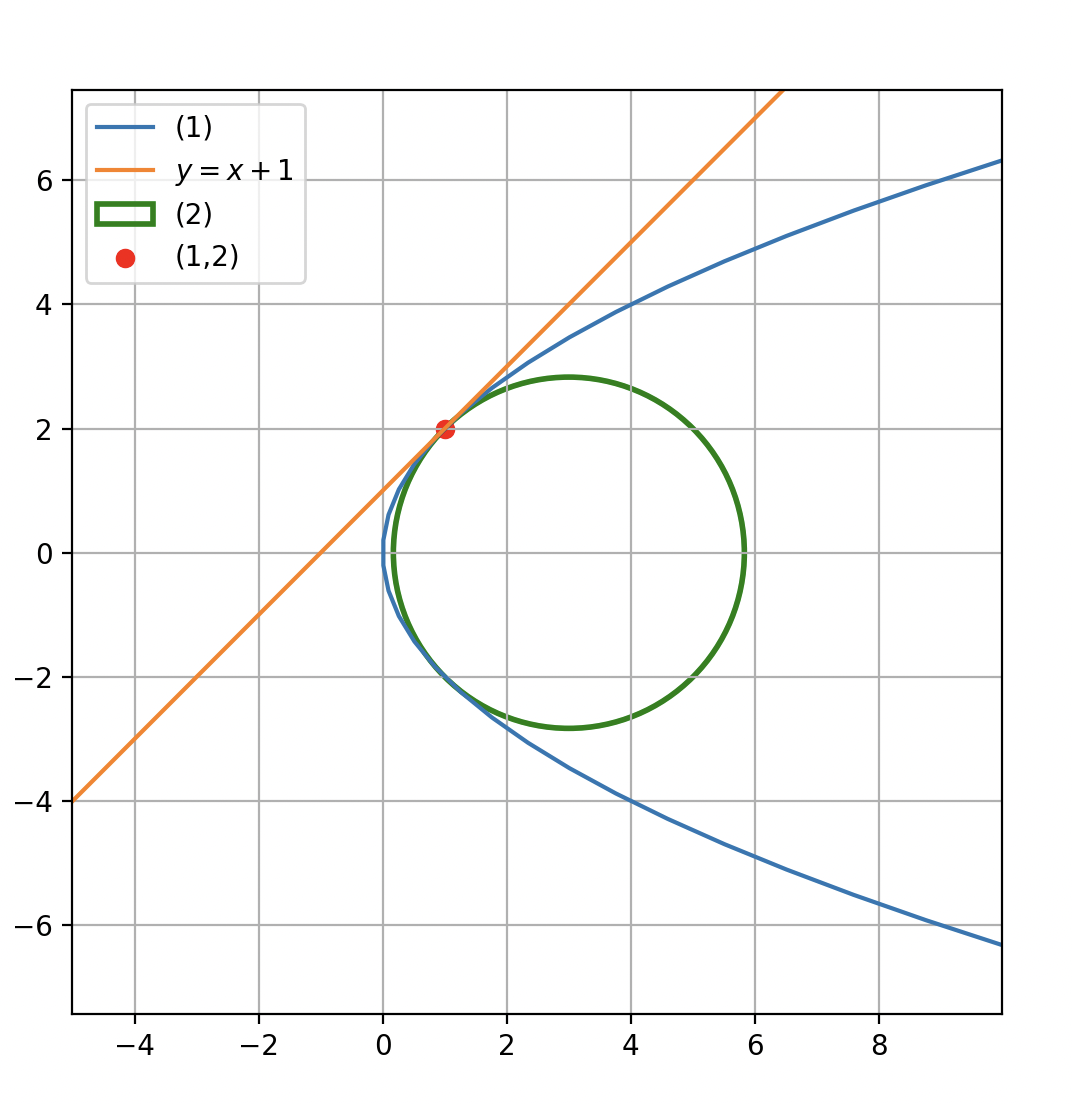
\includegraphics[width=0.5\columnwidth]{Figs/1032.png}
    \caption{Plot}
    \label{fig:placeholder}
\end{figure}
\end{frame}

\end{document}